% Template LaTeX document for CSSR4Africa Deliverables
% Adapted from documents prepared by EPFL for the RobotCub project
% and subsequently by the University of Skövde for the DREAM project
%
% DV 28/06/2023

\documentclass{CSSRforAfrica}

\usepackage[titletoc,title]{appendix}
\usepackage{dirtree}
\usepackage{graphicx}
\usepackage[hidelinks,colorlinks=false]{hyperref}
\usepackage{latexsym}
\usepackage{listings}
\usepackage{tikz}
\usepackage[table]{xcolor}

\usetikzlibrary{calc}
\usetikzlibrary{positioning}

\newcommand{\blank}{~\\}
\newcommand{\checkbox}{{~~~~~~~\leavevmode \put(-7,-1.5){  \huge $\Box$  }}}

\lstset{
    language=bash,
    basicstyle=\ttfamily\small,
    backgroundcolor=\color[rgb]{0.95, 0.95, 0.95},
    keywordstyle=\color[rgb]{0.1, 0.1, 0.8}\bfseries,
    commentstyle=\color[rgb]{0, 0.6, 0}\itshape,
    stringstyle=\color[rgb]{0.7, 0.1, 0.1},
    numbers=left,
    numberstyle=\color[rgb]{0.4, 0.4, 0.4}\tiny,
    stepnumber=1,
    numbersep=5pt,
    showspaces=false,
    showstringspaces=false,
    showtabs=false,
    tabsize=4,
    keepspaces=false,
    breakatwhitespace=false,
    breaklines=true,
    postbreak=\mbox{\textcolor{gray}{$\hookrightarrow$}\space},
    columns=fullflexible,
}



\begin{document}
\input{epsf}

%%
%% SHOULD NOT NEED TO BE CHANGED BEFORE THIS POINT
%% ------------------------------------------------
%%

\deliverable{D4.3.2}                   % REPLACE with correct number
\title{D4.3.2 Speech Event}    % REPLACE with correct title

\leadpartner{Carnegie Mellon University Africa}                        % INSERT partner name: Carnegie Mellon University Africa or The University of the Witwatersrand
\partner{The University of the Witwatersrand}                                % INSERT partner name: Carnegie Mellon University Africa or The University of the Witwatersrand

\revision{1.3}                          % REPLACE with correct version number
\deliverabledate{31/03/2024}   % REPLACE with correct date
\submissiondate{20/02/2025}  % REPLACE with correct date
\revisiondate{30/07/2025}                   % REPLACE with date
\disseminationlevel{PU}
\responsible{Clifford Onyonka}           % REPLACE with correct  name


%%
%% Create the titlepage
%%

\maketitle
 

\section*{Executive Summary}
%===============================================================
\label{executive_summary}
%%\addcontentsline{toc}{section}{Executive Summary}

Deliverable D4.3.2 concerns the results of Task 4.3.2, a task whose objective was to train, test, and finally deploy a speech-to-text model on a ROS node that will enable speech utterances in Kinyarwanda and English languages captured by Pepper's microphones to be transcribed into written text.

This report details the output of each phase of the software development process used in the fulfillment of Deliverable D4.3.2. The requirements definition section specifies the functional requirements of the users of Speech Event, the module specification section outlines the functional characteristics of Speech Event, the interface design section outlines the specification of the inputs and outputs of Speech Event, the module design section describes the deep neural networks that perform speech recognition of Kinyarwanda and English utterances, the testing section shows the results and descriptions of unit and end-to-end tests of Speech Event, and the user manual section outlines how to build and run Speech Event.

\newpage
 
 
%\graphicspath{{./figs/}}
\pagebreak
\tableofcontents
\newpage


\section{Introduction}
%===============================================================
Conversational systems are developed using the following main components: automatic speech recognition (speech-to-text), natural language understanding, dialogue manager, natural language generation, and text-to-speech. Speech-to-text converts an audio signal containing spoken speech utterances to written text transcriptions, natural language understanding analyses the transcribed text to extract meaning, the dialogue manager generates a response based on the inferred meaning of the text, natural language generation formulates text based on the response generated by the dialogue manager, and text-to-speech synthesises spoken speech utterances to be played to the other agent(s) in the conversation cycle \cite{romero-gonzalez_spoken_2020}. Such a system is displayed in Fig \ref{fig:conversational-system}.

\begin{figure}[thb]
\begin{center}
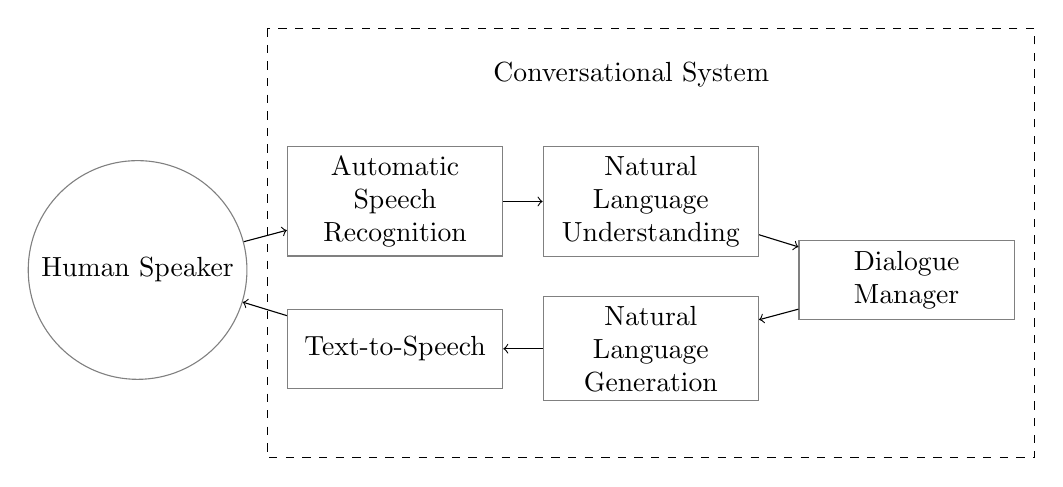
\begin{tikzpicture}
    \node [rectangle, minimum size=1cm, text width=2.5cm, anchor=base, draw=black!50, text centered] (asr) {Automatic Speech Recognition} node[above=1cm, xshift=3cm] {Conversational System};
    \node [rectangle, minimum size=1cm, text width=2.5cm, anchor=base, draw=black!50, text centered, right=0.5cm of asr] (nlu) {Natural Language Understanding};
    \node [rectangle, minimum size=1cm, text width=2.5cm, anchor=base, draw=black!50, text centered, right=0.5cm of nlu, yshift=-1cm] (dm) {Dialogue Manager};
    \node [rectangle, minimum size=1cm, text width=2.5cm, anchor=base, draw=black!50, text centered, below=0.5cm of nlu] (nlg) {Natural Language Generation};
    \node [rectangle, minimum size=1cm, text width=2.5cm, anchor=base, draw=black!50, text centered, left=0.5cm of nlg] (tts) {Text-to-Speech};
    \node[circle, minimum size=1cm, text width=2.5cm, anchor=base, draw=black!50, text centered, left=0.5cm of tts, yshift=1cm] (agent) {Human Speaker};
    \draw[dashed] ([xshift=-0.25cm, yshift=1.5cm] asr.north west) rectangle ([xshift=0.25cm, yshift=-1.75cm] dm.south east);

    \draw [->] (agent) -- (asr);
    \draw [->] (asr) -- (nlu);
    \draw [->] (nlu) -- (dm);
    \draw [->] (dm) -- (nlg);
    \draw [->] (nlg) -- (tts);
    \draw [->] (tts) -- (agent);
\end{tikzpicture}
\end{center}
\caption{A diagrammatic representation of a conversational system \cite{romero-gonzalez_spoken_2020}}
\label{fig:conversational-system}
\end{figure}
 
The Speech Event module only handles one component of the conversational system described in the previous paragraph, that is, speech-to-text (which is referred to as automatic speech recognition in Fig \ref{fig:conversational-system}). It acquires audio signals published on the \texttt{/soundDetection/signal} ROS topic, and then passes these audio signals through a deep neural network that transcribes speech utterances contained within the audio to generate text string representations, which are then published on the \texttt{/speechEvent/text} ROS topic. Kinyarwanda and English are the two languages that are transcribed by Speech Event, with the choice of language being set by the Behaviour Controller which reads it from the Culture Knowledge Base and then passes it to Speech Event via the \texttt{/speechEvent/set\_language} ROS service that is advertised by Speech Event.


\newpage
\section{Requirements Definition}
%===============================================================
A running Speech Event ROS node performs one main function - Kinyarwanda and English speech recognition. An audio signal is received via the \texttt{/soundDetection/signal} ROS topic, and Speech Event transcribes any speech utterances detected in the signal to either Kinyarwanda or English.

In order to successfully perform this function, the following functional requirements are fulfilled by Speech Event:

\begin{enumerate}
    \item Acquire an audio signal from the \texttt{/soundDetection/signal} ROS topic
    \item Pass the audio signal through an automatic speech recognition (ASR) model to transcribe any speech utterances the audio signal contains to either Kinyarwanda or English text
    \item Publish the transcribed text to the \texttt{/speechEvent/text} ROS topic
\end{enumerate}

The exact language between Kinyarwanda and English, which a running Speech Event ROS node transcribes, is decided based on a configuration option that is set during the initialisation stage when the ROS node is started. The language that is set during the initialisation of the Speech Event ROS node can be overridden by invoking the \texttt{/speechEvent/set\_language} ROS service and passing a different language to it.

To supplement the core functionality that Speech Event performs (Kinyarwanda and English speech recognition), the text transcriptions that Speech Event transcribes are displayed on a graphical interface. The graphical interface is used as a replacement for the terminal interface, especially in presentation settings where displaying text transcriptions on the terminal is impractical due to the small font size used by the terminal and the extra verbosity of the results displayed on the terminal. This graphical interface is enabled when the ROS node is configured to run in verbose mode.

A ROS node that emulates Sound Detection is also availed, and its main purpose is to showcase the working of Speech Event in isolation, separated from the rest of the CSSR4Africa system and from the Pepper robot. This ROS node captures audio from the computer on which Speech Event is running on, and publishes the captured audio to the same ROS topic that Sound Detection publishes to (\texttt{/soundDetection/signal}), therefore mimicking Sound Detection's operation of acquiring audio from Pepper and publishing it to the aforementioned ROS topic.

A ROS service is also be provided for enabling and disabling the transcription process at runtime. This ROS service \texttt{/speechEvent/set\_enabled} is invoked by the Behaviour Controller to disable the transcription process when Pepper is speaking so as to avoid the transcription of Pepper's utterances, and then re-enabling the transcription process once Pepper is no longer speaking.

It is also worth noting that Sound Detection may fail, and since the Behaviour Controller does not directly interface with Sound Detection, the Speech Event ROS node bears the burden of signaling failures that may arise in Sound Detection to the Behaviour Controller. This is done by publishing the message `Error: soundDetection is down' on the \texttt{/speechEvent/text} ROS topic.


\newpage
\section{Module Specification}
%===============================================================
A running Speech Event ROS node performs speech-to-text in real-time, acquiring an audio signal from the \texttt{/soundDetection/signal} ROS topic, generating a text description of the acquired audio, and then publishing transcribed text to the \texttt{/speechEvent/text} ROS topic as soon as speech utterances are detected in the audio signal. The data that is input to Speech Event, the transformation that this data undergoes, and the data that Speech Event outputs is described below:

\begin{enumerate}
    \item The language that Speech Event is to be configured to operate in is set when the ROS node is started by setting a language configuration option
    \item The language set for Speech Event to operate in when it is first started can be overridden by making a \texttt{/speechEvent/set\_language} ROS service call and passing a different language
    \item When the Speech Event ROS node is running, it acquires audio signals published by the Sound Detection ROS node on the \texttt{/soundDetection/signal} ROS topic
    \item The acquired audio signals are then passed through an ASR model that transcribes speech utterances present within the audio signals to text strings
    \item The text strings output by the ASR model are then published to the \texttt{/speechEvent/text} ROS topic for the Behaviour Controller to use
    \item The transcription process can be enabled or disabled by invoking the \texttt{/speechEvent/set\_enabled} ROS service
\end{enumerate}

This process, and the position of Speech Event within the CSSR4Africa system architecture, is captured in Fig \ref{fig:speechEvent-within-CSSR4A}.

\begin{figure}[thb]
\begin{center}
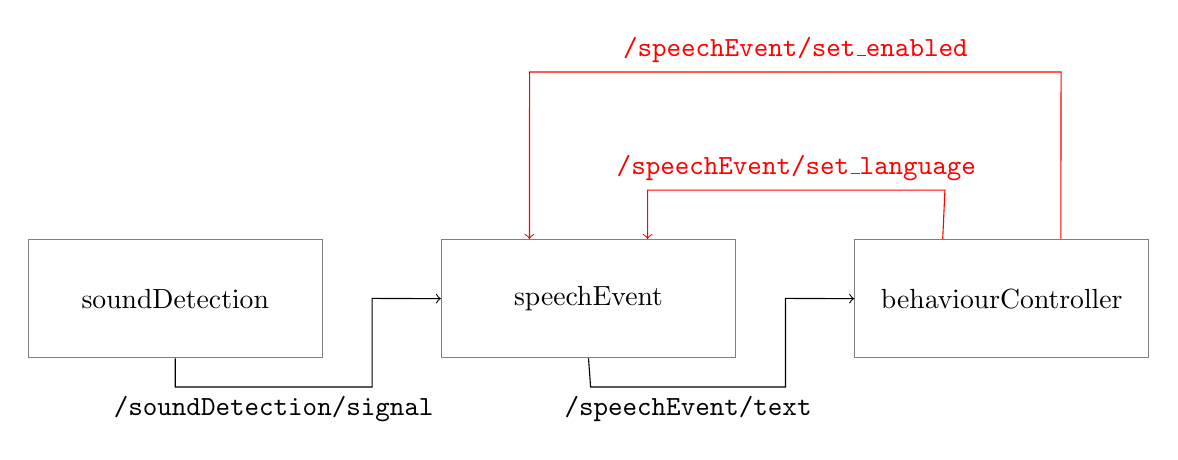
\begin{tikzpicture}
    \node [rectangle, minimum size=1.5cm, text width=3.5cm, anchor=base, draw=black!50, text centered] (soundDetection) {soundDetection};
    \node [rectangle, minimum size=1.5cm, text width=3.5cm, anchor=base, draw=black!50, text centered, right=1.5cm of soundDetection] (speechEvent) {speechEvent};  
    \node [rectangle, minimum size=1.5cm, text width=3.5cm, anchor=base, draw=black!50, text centered, right=1.5cm of speechEvent] (behaviourController) {behaviourController};

    \draw [->] (soundDetection.south) -- (0, -1) -- (2.5, -1) node[pos=0.5, below] {\texttt{/soundDetection/signal}} -- (2.5, 0.125) -- (speechEvent.west);
    \draw [->] (speechEvent.south) -- (5.275, -1) -- (7.75, -1) node[pos=0.5, below] {\texttt{/speechEvent/text}} -- (7.75, 0.125) -- (behaviourController.west);
    \draw [->, red] ($(behaviourController.north)+(-0.75cm,0)$) -- (9.775, 1.5) -- (6, 1.5) node[pos=0.5, above] {\texttt{/speechEvent/set\_language}} -- ($(speechEvent.north)+(0.75cm,0)$);
    \draw [->, red] ($(behaviourController.north)+(+0.75cm,0)$) -- (11.25, 3) -- (4.5, 3) node[pos=0.5, above] {\texttt{/speechEvent/set\_enabled}} -- ($(speechEvent.north)+(-0.75cm,0)$);
\end{tikzpicture}
\end{center}
\caption{Speech Event within the CSSR4Africa architecture (\texttt{/soundDetection/signal} and \texttt{/speechEvent/text} are ROS topics, \textcolor{red}{\texttt{/speechEvent/set\_language}} and \textcolor{red}{\texttt{/speechEvent/set\_enabled}} are ROS services)}
\label{fig:speechEvent-within-CSSR4A}
\end{figure}


\newpage
\section{Interface Design}
%===============================================================
\subsection{Source Code}
The file structure of Speech Event is as shown below:

\vspace{1cm}
\dirtree{%
.1 speech\_event/.
.2 config/.
.3 speech\_event\_configuration.ini.
.2 data/.
.3 audio\_storage/.
.3 pepper\_topics.dat.
.2 models/.
.3 stt\_en\_conformer\_transducer\_large.nemo.
.3 stt\_rw\_conformer\_transducer\_large.nemo.
.2 src/.
.3 speech\_event\_application.py.
.3 speech\_event\_implementation.py.
.2 srv/.
.3 set\_enabled.srv.
.3 set\_language.srv.
.2 README.md.
.2 speech\_event\_requirements.txt.
}
\vspace{1cm}

The \texttt{config/} directory houses configuration files that are used to configure different ROS nodes that are part of Speech Event. For Speech Event, only the \texttt{speech\_event\_configuration.ini} file exists in this directory, and it is used to configure the main Speech Event ROS node.

The \texttt{data/} directory contains data that is required by Speech Event when running. For Speech Event, the \texttt{pepper\_topics.dat} file and \texttt{audio\_storage/} sub-directory are contained in this directory:

\begin{enumerate}
    \item \texttt{pepper\_topics.dat}: list of ROS topics that Speech Event listens to when it is running
    \item \texttt{audio\_storage}: stores temporary audio files generated when Speech Event is transcribing speech utterances
\end{enumerate}

The \texttt{models/} directory holds the two deep learning models used to transcribe speech utterances:

\begin{enumerate}
    \item \texttt{stt\_rw\_conformer\_transducer\_large.nemo} for transcribing Kinyarwanda utterances
    \item \texttt{stt\_en\_conformer\_transducer\_large.nemo} for transcribing English utterances
\end{enumerate}

The \texttt{src/} directory holds all the Python source code files that implement the Speech Event system.

The \texttt{srv/} directory contains the \texttt{set\_language.srv} service file specification for the ROS service \texttt{/speechEvent/set\_language} and the \texttt{set\_enabled.srv} service file specification for the ROS service \texttt{/speechEvent/set\_enabled} .

The file \texttt{README.md} contains documentation of how to use Speech Event,  and the Python requirements file \texttt{speech\_event\_requirements.txt} contains a list of versioned Python packages that Speech Event depends on.

\subsection{Configuration Files}

A Speech Event ROS node needs to be configured prior to starting it, a task that is accomplished via a configuration file. The configuration parameters are displayed in Table \ref{table:speechEvent-config-file}.

\begin{center}
\begin{table}[thb]
\begin{tabular}[thb]{|p{0.27\linewidth}|p{0.20\linewidth}|p{0.45\linewidth}|}\hline
\rowcolor{lightgray} Key & Value & Description \\ \hline
\texttt{language} & \texttt{kinyarwanda}, \texttt{english} & Specifies the language in which the utterance is spoken. \\ \hline
\texttt{verboseMode} & \texttt{true}, \texttt{false} & Specifies whether diagnostic data is to be printed to the terminal. \\ \hline
\texttt{cuda} & \texttt{true}, \texttt{false} & Specifies whether to use GPUs. The term ‘cuda’ is chosen as the key to alert the user that only NVIDIA GPUs are supported. \\ \hline
\texttt{confidence} & \texttt{<float>} & The confidence level on a scale of 0 to 1 above which transcriptions are assumed to be acceptable and correct. \\ \hline
\texttt{speechPausePeriod} & \texttt{<float>} & The time period above which one utterance is assumed to be separate from a preceding utterance. \\ \hline
\texttt{maxUtteranceLength} & \texttt{<integer>} & The maximum length (in seconds) of an utterance. Longer utterances are split when they go past this length. \\ \hline
\texttt{sampleRate} & \texttt{<integer>} & Specifies the sampling rate of the incoming audio sourced from the /soundDetection/signal ROS topic. \\ \hline
\texttt{heartbeatMsgPeriod} & \texttt{<integer>} & Specifies the time period in seconds at which a periodic heartbeat message is sent to the terminal. \\ \hline
\end{tabular}
\caption{Speech Event configuration file options}
\label{table:speechEvent-config-file}
\end{table}
\end{center}

\subsection{Data Files}

The topics that Speech Event subscribes to are listed in the \texttt{pepper\_topics.dat} file, as shown in Table \ref{table:speechEvent-topics-file}.

\begin{center}
\begin{table}[thb]
\begin{tabular}[thb]{|p{0.31\linewidth}|p{0.60\linewidth}|}\hline
\rowcolor{lightgray} Key & Value \\ \hline
\texttt{soundDetection} & \texttt{/soundDetection/signal} \\ \hline
\end{tabular}
\caption{ROS topics that Speech Event subscribes to}
\label{table:speechEvent-topics-file}
\end{table}
\end{center}

\newpage
\subsection{Topics Subscribing To}

A running Speech Event ROS node acquires audio signals from the \texttt{/soundDetection/signal} ROS topic. Table \ref{table:topics-sub} shows this fact, while also mentioning the ROS node that publishes these audio signals.

\begin{center}
\begin{table}[thb]
\begin{tabular}[thb]{|p{0.32\linewidth}|p{0.30\linewidth}|p{0.28\linewidth}|} \hline
\rowcolor{lightgray} Topic & Node & Platform \\ \hline
\texttt{/soundDetection/signal} & \texttt{soundDetection} & \texttt{Physical robot} \\ \hline
\end{tabular}
\caption{Topics subscribing to}
\label{table:topics-sub}
\end{table}
\end{center}

\subsection{Topics Publishing To}

The Speech Event ROS node publishes transcribed text to the \texttt{/speechEvent/text} ROS topic, publishing each time a transcription process completes. The published text transcriptions are of the \texttt{string} data type. Table \ref{table:topics-pub} shows the ROS topic that Speech Event publishes to.

\begin{center}
\begin{table}[thb]
\begin{tabular}[thb]{|p{0.30\linewidth}|p{0.30\linewidth}|p{0.30\linewidth}|} \hline
\rowcolor{lightgray} Topic & Node & Platform \\ \hline
\texttt{/speechEvent/text} & \texttt{behaviourController} & \texttt{Physical robot} \\ \hline
\end{tabular}
\caption{Topics publishing to}
\label{table:topics-pub}
\end{table}
\end{center}

\subsection{Services Supported}

A running Speech Event ROS node can have its language of operation (Kinyarwanda or English) updated by invoking the \texttt{/speechEvent/set\_language} ROS service, or enabled or disabled at runtime by invoking the \texttt{/speechEvent/set\_enabled} ROS service. Table \ref{table:services} elaborates these ROS services.

\begin{center}
\begin{table}[thb]
\begin{tabular}[thb]{|p{0.36\linewidth}|p{0.18\linewidth}|p{0.36\linewidth}|} \hline
\rowcolor{lightgray} Service & Message Value & Effect \\ \hline
\texttt{/speechEvent/set\_enabled} & \texttt{true}, \texttt{false} & Enable or disable the transcription process \\ \hline
\texttt{/speechEvent/set\_language} & \texttt{kinyarwanda}, \texttt{english} & Set the language to either Kinyarwanda or English \\ \hline
\end{tabular}
\caption{Services supported}
\label{table:services}
\end{table}
\end{center}


\newpage
\section{Module Design}
%===============================================================
\subsection{Model Architecture}
Both the Kinyarwanda and English speech recognition processes performed by Speech Event rely on deep learning models. Both of these deep learning models are based on the conformer transducer architecture, and the specific models that are used by Speech Event were acquired from NVIDIA's Nemo catalog of models.

The conformer transducer architecture is made up of a conformer encoder and a transducer decoder. The conformer encoder combines transformers and Convolution Neural Networks (CNNs) in an attempt to utilise the strengths of both, with transformers excelling at capturing global dependencies of an audio signal and CNNs excelling at capturing local dependencies of an audio signal \cite{gulati_conformer_2020}. The transducer decoder, on the other hand, makes use of Recurrent Neural Networks (RNNs) to form an autoregressive model whose next token prediction is conditioned on the previously predicted tokens.

\subsubsection{Preprocessor}
When an audio signal is received, it is first passed through a preprocessor block that extracts filterbank features from the audio signal. For this process, an audio signal is first converted to a spectrogram by a Short Time Fourier Transform (STFT), and then a series of filters is applied to the resultant spectrogram to obtain the filterbank features that each represent the magnitude of the energy within a distinct frequency band. This preprocessor block is visualised in Fig \ref{fig:preprocessor}.

\begin{figure}[thb]
\begin{center}
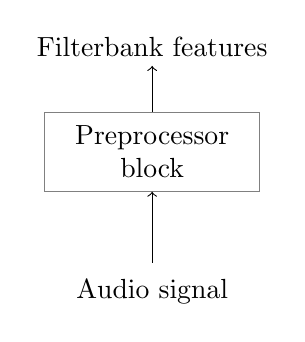
\begin{tikzpicture}
    \node [rectangle, minimum size=1cm, text width=2.5cm, anchor=base, draw=black!50, text centered] (preprocessor) {Preprocessor block};

    \draw [->] (0, -1.5) -- (preprocessor) node[below=1.5cm] {Audio signal};
    \draw [->] (preprocessor) -- (0, 1) node[above=0cm] {Filterbank features};
\end{tikzpicture}
\end{center}
\caption{Audio to filterbank features preprocessor}
\label{fig:preprocessor}
\end{figure}

\subsubsection{Encoder Architecture}
The filterbank features obtained from the preprocessor block are then passed to the encoder part of the model. The encoder transforms acoustic features in the original audio signal captured within the filterbank features into latent features that better represent the speech in the original audio signal.

A conformer encoder is shown in Fig \ref{fig:conformer-encoder}. The encoder used in Speech Event has 17 conformer blocks.

\begin{figure}[thb]
\begin{center}
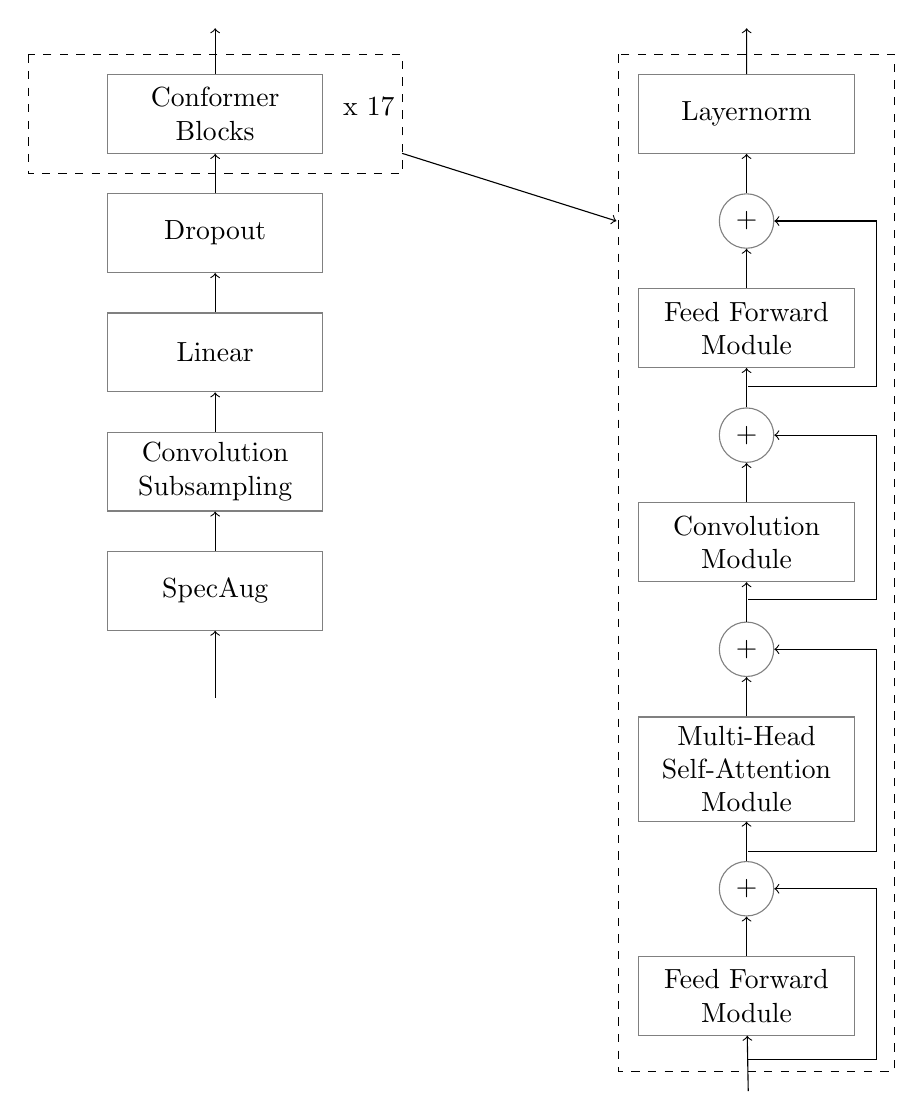
\begin{tikzpicture}
    \node [rectangle, minimum size=1cm, text width=2.5cm, anchor=base, draw=black!50, text centered] (conformer_blocks) {Conformer Blocks} node[right=1.5cm] {x 17};
    \node [rectangle, minimum size=1cm, text width=2.5cm, anchor=base, draw=black!50, text centered, below=0.5cm of conformer_blocks] (dropout) {Dropout};
    \node [rectangle, minimum size=1cm, text width=2.5cm, anchor=base, draw=black!50, text centered, below=0.5cm of dropout] (linear) {Linear};
    \node [rectangle, minimum size=1cm, text width=2.5cm, anchor=base, draw=black!50, text centered, below=0.5cm of linear] (conv_subsamp) {Convolution Subsampling};
    \node [rectangle, minimum size=1cm, text width=2.5cm, anchor=base, draw=black!50, text centered, below=0.5cm of conv_subsamp] (spec_aug) {SpecAug};
    \draw[dashed] ([xshift=-1cm, yshift=0.25cm] conformer_blocks.north west) rectangle ([xshift=1cm, yshift=-0.25cm] conformer_blocks.south east);

    \draw [->] (0, -7.5) -- (spec_aug);
    \draw [->] (spec_aug) -- (conv_subsamp);
    \draw [->] (conv_subsamp) -- (linear);
    \draw [->] (linear) -- (dropout);
    \draw [->] (dropout) -- (conformer_blocks);
    \draw [->] (conformer_blocks) -- (0, 1);

    \node [rectangle, minimum size=1cm, text width=2.5cm, anchor=base, draw=black!50, text centered, right=4cm of conformer_blocks] (layernorm) {Layernorm};
    \node[circle, anchor=base, draw=black!50, text centered, below=0.5cm of layernorm] (plus4) {+};
    \node [rectangle, minimum size=1cm, text width=2.5cm, anchor=base, draw=black!50, text centered, below=0.5cm of plus4] (ff_module2) {Feed Forward Module};
    \node[circle, anchor=base, draw=black!50, text centered, below=0.5cm of ff_module2] (plus3) {+};
    \node [rectangle, minimum size=1cm, text width=2.5cm, anchor=base, draw=black!50, text centered, below=0.5cm of plus3] (conv_module) {Convolution Module};
    \node[circle, anchor=base, draw=black!50, text centered, below=0.5cm of conv_module] (plus2) {+};
    \node [rectangle, minimum size=1cm, text width=2.5cm, anchor=base, draw=black!50, text centered, below=0.5cm of plus2] (selt_attention) {Multi-Head Self-Attention Module};
    \node[circle, anchor=base, draw=black!50, text centered, below=0.5cm of selt_attention] (plus1) {+};
    \node [rectangle, minimum size=1cm, text width=2.5cm, anchor=base, draw=black!50, text centered, below=0.5cm of plus1] (ff_module1) {Feed Forward Module};
    \draw[dashed] ([xshift=-0.25cm, yshift=0.25cm] layernorm.north west) rectangle ([xshift=0.5cm, yshift=-0.45cm] ff_module1.south east);

    \draw [->] (6.77, -12.5) -- (ff_module1);
    \draw [->] (ff_module1) -- (plus1);
    \draw [->] (plus1) -- (selt_attention);
    \draw [->] (selt_attention) -- (plus2);
    \draw [->] (plus2) -- (conv_module);
    \draw [->] (conv_module) -- (plus3);
    \draw [->] (plus3) -- (ff_module2);
    \draw [->] (ff_module2) -- (plus4);
    \draw [->] (plus4) -- (layernorm);
    \draw [->] (layernorm) -- (6.75, 1);

    \draw[->] (6.77, -12.1) -| (8.4, -12.1) |- (plus1.east);
    \draw[->] (6.77, -9.45) -| (8.4, -9.45) |- (plus2.east);
    \draw[->] (6.77, -6.25) -| (8.4, -6.25) |- (plus3.east);
    \draw[->] (6.77, -3.55) -| (8.4, -3.55) |- (plus4.east);

    \coordinate (start) at ($(conformer_blocks.east)+(1cm, -0.5cm)$);
    \coordinate (end) at ($(plus4.west)+(-1.3cm, 0)$);
    \draw [->] (start) -- (end);
\end{tikzpicture}
\end{center}
\caption{Conformer encoder architecture \cite{gulati_conformer_2020}}
\label{fig:conformer-encoder}
\end{figure}

The filterbank features are first passed through a SpecAugment block. SpecAugment is a data augmentation method that is suitable for end-to-end speech recognition models such as the Conformer Transducer model used by Speech Event. ``The augmentation policy consists of warping the features, masking blocks of frequency channels, and masking blocks of time steps'' \cite{park_specaugment_2019}.

The features are then processed by a convolution subsampling block, dropout applied, and then passed through a series of 17 conformer blocks in the encoder.

Each confomer block consists of a multi-head self-attention module and a convolution module collectively sandwiched between two feedforward modules \cite{gulati_conformer_2020}. The self-attention module is more adept at capturing global feature dependencies, while the convolution module is more adept at capturing local feature dependencies, thereby capturing the semantics of speech utterances much better than models that only specialise in capturing only one of either the global or local feature dependencies.

\subsubsection{Decoder/Predictor Architecture}
Keeping in line with Gulati et al., a single LSTM layer is used in the decoder \cite{gulati_conformer_2020}. An embedding layer converts input tokens into vectorised representations that are then passed to the LSTM layer. Additionally, drop out is applied both in the LSTM layer and on the output of the LSTM layer.

The decoder architecture used in Speech Event is shown in Fig \ref{fig:transducer-decoder}.

\begin{figure}[thb]
\begin{center}
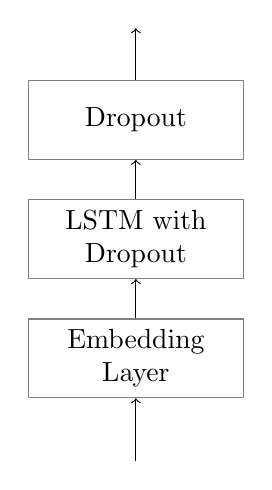
\begin{tikzpicture}
    \node [rectangle, minimum size=1cm, text width=2.5cm, anchor=base, draw=black!50, text centered] (dropout) {Dropout};
    \node [rectangle, minimum size=1cm, text width=2.5cm, anchor=base, draw=black!50, text centered, below=0.5cm of dropout] (lstm) {LSTM with Dropout};
    \node [rectangle, minimum size=1cm, text width=2.5cm, anchor=base, draw=black!50, text centered, below=0.5cm of lstm] (embedding) {Embedding Layer};

    \draw [->] (0, -4.25) -- (embedding);
    \draw [->] (embedding) -- (lstm);
    \draw [->] (lstm) -- (dropout);
    \draw [->] (dropout) -- (0, 1.25);
\end{tikzpicture}
\end{center}
\caption{Transducer predictor architecture}
\label{fig:transducer-decoder}
\end{figure}

\subsubsection{Joint Network Architecture}
The joint network combines the output of the encoder and the output of the decoder in order to predict the text in the speech utterances contained in the original sound signal passed to the encoder. The combined outputs are then passed through a ReLU activation, dropout is applied, and lastly passed through a linear layer.

The joint network architecture used in Speech Event is shown in Fig \ref{fig:joint}.

\begin{figure}[thb]
\begin{center}
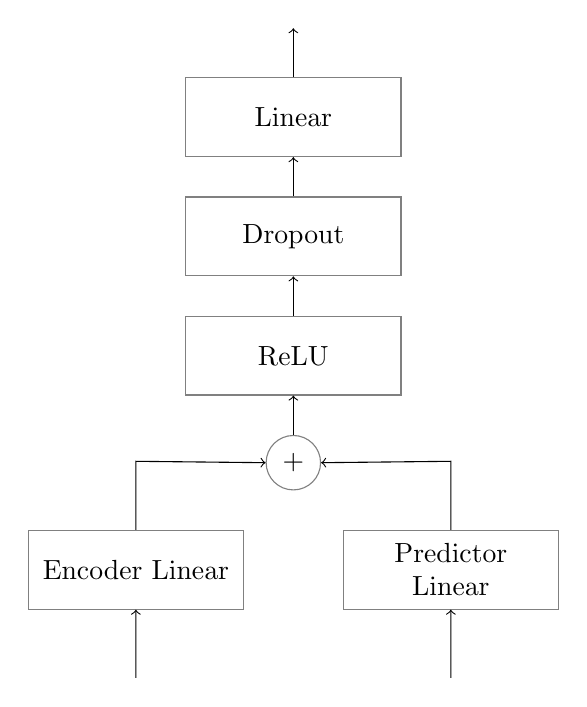
\begin{tikzpicture}
    \node [rectangle, minimum size=1cm, text width=2.5cm, anchor=base, draw=black!50, text centered] (linear) {Linear};
    \node [rectangle, minimum size=1cm, text width=2.5cm, anchor=base, draw=black!50, text centered, below=0.5cm of linear] (dropout) {Dropout};
    \node [rectangle, minimum size=1cm, text width=2.5cm, anchor=base, draw=black!50, text centered, below=0.5cm of dropout] (relu) {ReLU};
    \node[circle, anchor=base, draw=black!50, text centered, below=0.5cm of relu] (plus) {+};
    \node [rectangle, minimum size=1cm, text width=2.5cm, anchor=base, draw=black!50, text centered, below=0.5cm of plus, xshift=-2cm] (enc) {Encoder Linear};
    \node [rectangle, minimum size=1cm, text width=2.5cm, anchor=base, draw=black!50, text centered, below=0.5cm of plus, xshift=2cm] (pred) {Predictor Linear};

    \draw [->] (-2, -7) -- (enc);
    \draw [->] (2, -7) -- (pred);
    \draw [->] (enc.north) -- (-2, -4.25) -- (plus.west);
    \draw [->] (pred.north) -- (2, -4.25) -- (plus.east);
    \draw [->] (plus) -- (relu);
    \draw [->] (relu) -- (dropout);
    \draw [->] (dropout) -- (linear);
    \draw [->] (linear) -- (0, 1.25);
\end{tikzpicture}
\end{center}
\caption{Joint architecture}
\label{fig:joint}
\end{figure}

\subsubsection{Combined Model Architecture}
The four different sections of the full conformer transducer architecture discussed above are combined together to form the whole network that performs end-to-end automatic speech recognition. This full model's architecture is summaried in Fig \ref{fig:combined}.

\begin{figure}[thb]
\begin{center}
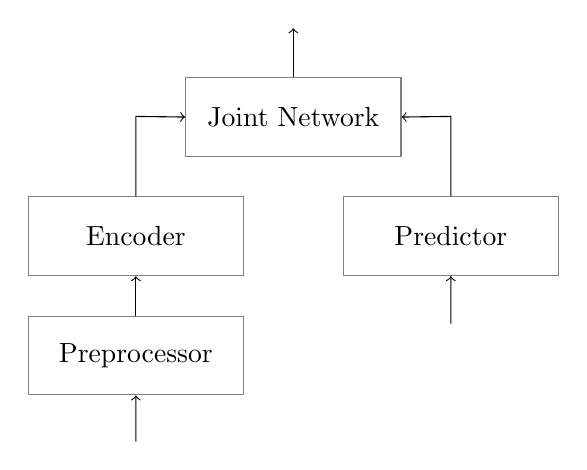
\begin{tikzpicture}
    \node [rectangle, minimum size=1cm, text width=2.5cm, anchor=base, draw=black!50, text centered] (joint) {Joint Network};
    \node [rectangle, minimum size=1cm, text width=2.5cm, anchor=base, draw=black!50, text centered, below=0.5cm of joint, xshift=-2cm] (encoder) {Encoder};
    \node [rectangle, minimum size=1cm, text width=2.5cm, anchor=base, draw=black!50, text centered, below=0.5cm of joint, xshift=2cm] (decoder) {Predictor};
    \node [rectangle, minimum size=1cm, text width=2.5cm, anchor=base, draw=black!50, text centered, below=0.5cm of encoder] (preprocessor) {Preprocessor};

    \draw [->] (-2, -4) -- (preprocessor);
    \draw [->] (2, -2.5) -- (decoder);
    \draw [->] (preprocessor) -- (encoder);
    \draw [->] (encoder.north) -- (-2, 0.13) -- (joint.west);
    \draw [->] (decoder.north) -- (2, 0.13) -- (joint.east);
    \draw [->] (joint) -- (0, 1.25);
\end{tikzpicture}
\end{center}
\caption{Combined model architecture}
\label{fig:combined}
\end{figure}


\newpage
\section{Testing}
%===============================================================
The \texttt{unit\_tests} package contains unit tests for all CSSR4Africa ROS nodes, including Speech Event. Python's unittest testing framework is used for testing. The unittest package is part of the standard Python library, and therefore no extra packages need to be installed when running tests.

These tests check to ensure that Speech Event works as expected end-to-end, from when it receives a signal on the \texttt{/soundDetection/signal} ROS topic to when it publishes transcribed text on the \texttt{/speechEvent/text} ROS topic. They also check that the \texttt{/speechEvent/set\_language} and \texttt{/speechEvent/set\_enabled} ROS services work as expected.

A test report is generated in the \texttt{data/} directory, \texttt{speech\_event\_test\_output.dat}. It shows all the tests that have been run and whether they have passed or failed. For tests that err, the reason for the error is also shown within the test report.

Before running tests, the ROS node that runs these tests has to be configured. The driver ROS node that emulates the Sound Detection ROS node also has to be configured, if the tests will not be run using the Pepper robot.

The configuration options for the ROS node that runs the tests are located in the configuration file \texttt{speech\_event\_test\_configuration.ini}. They are shown in Table \ref{table:test-configuration}.

\begin{center}
\begin{table}[thb]
\begin{tabular}[thb]{|p{0.27\linewidth}|p{0.20\linewidth}|p{0.45\linewidth}|} \hline
\rowcolor{lightgray} Key & Value & Description \\ \hline
\texttt{heartbeatMsgPeriod} & \texttt{<integer>} & Specifies the time period in seconds at which
a periodic heartbeat message is sent to the terminal. \\ \hline
\texttt{waitTimeout} & \texttt{<integer>} & Specifies how long to wait for speechEvent to start. \\ \hline
\texttt{mode} & \texttt{mic}, \texttt{file} & Use `mic' when using real-time utterances from Pepper or the driver ROS node, and `file' when using saved audio files. \\ \hline
\end{tabular}
\caption{Speech Event Test configuration file}
\label{table:test-configuration}
\end{table}
\end{center}

When using a driver ROS node, the following is important when configuring the driver ROS node:

\begin{itemize}
    \item Tweak the \texttt{speechAmplitudeThreshold} in case the driver is having trouble capturing speech utterances. Increase it in case speech is not being detected, and decrease it in case ambient noise is being captured together with the speech utterances. You may also tweak the sensitivity of the PC's microphones in case \texttt{sspeechAmplitudeThreshold} fails to solve the aforementioned issues that may arise.
    \item When using the driver to test Speech Event, ensure that \texttt{mode} in the driver configuration file matches \texttt{mode} in Speech Event Test configuration file (either set both to \texttt{file} or set both to \texttt{mic}). When using a running Sound Detection ROS node to test Speech Event, ensure that \texttt{mode} in the Speech Event Test configuration is set to \texttt{mic}.
    \item If using ROS launch files to launch the test harness, the argument passed to the \texttt{mode} parameter of the launch file will override whatever is set in the configuration files. Therefore when using the test harness launch file, no need to update the \texttt{mode} option in the configuration files, as setting it once while launching using the test harness launch file suffices.
\end{itemize}

The configuration options for the driver ROS node are located in the driver configuration file \texttt{speech\_event\_driver\_configuration.ini}. They are shown in Table \ref{table:driver-configuration}.

\begin{center}
\begin{table}[thb]
\begin{tabular}[thb]{|p{0.35\linewidth}|p{0.13\linewidth}|p{0.44\linewidth}|} \hline
\rowcolor{lightgray} Key & Value & Description \\ \hline
\texttt{channels} & \texttt{<integer>} & Number of audio channels to use when acquiring audio from PC's microphones. \\ \hline
\texttt{chunkSize} & \texttt{<integer>} & Number of samples to acquire at a go every time that audio is read from the PC's microphones. \\ \hline
\texttt{sampleRate} & \texttt{<integer>} & The sample rate to use when acquiring audio from the PC's microphones. \\ \hline
\texttt{speechAmplitudeThreshold} & \texttt{<float>} & Threshold above which a signal sample is assumed to contain a speech utterance. \\ \hline
\texttt{mode} & \texttt{mic}, \texttt{file} & Use `mic' when using real-time utterances from Pepper or the driver ROS node, and `file' when using saved audio files. \\ \hline
\end{tabular}
\caption{Speech Event Driver configuration file}
\label{table:driver-configuration}
\end{table}
\end{center}

The tests for Speech Event test the following:

\begin{enumerate}
    \item The working of the \texttt{/speechEvent/set\_enabled} ROS service
    \item The working of the \texttt{/speechEvent/set\_language} ROS service
    \item The end-to-end working of Speech Event as a whole, from when an audio signal is received from the \texttt{/soundDetection/signal} ROS topic to when a text transcription is published on the \texttt{/speechEvent/text} ROS topic
\end{enumerate}

A sample test report that is generated at the end of each testing process is displayed below (some lines have been artificially folded to the next line in this report to avoid overflowing out of the page):

\begin{verbatim}
Speech Event Test Report
    
Date: 2025-04-20 18:34:47
    
    
====================================================================
    
Test SpeechEvent's /speechEvent/set_enabled ROS service
---
As a:     behaviourController developer
I want:   a means of enabling and disabling the transcription process
          at runtime
So that:  I can stop the robot from transcribing its own speech by
          disabling the transcription process
---
Set unsupported status (agree): PASS
Set unsupported status (1): PASS
Set supported status (false): PASS
Set supported status (true): PASS

====================================================================

Test SpeechEvent's /speechEvent/set_language ROS service
---
As a:     behaviourController developer
I want:   a means of setting the transcription language of
          speechEvent at runtime
So that:  I don't have to restart speechEvent every time I update the
          transcription language
---
Set unsupported language (Kiswahili): PASS
Set unsupported language (Arabic): PASS
Set supported language (English): PASS
Set supported language (Kinyarwanda): PASS

====================================================================

Test SpeechEvent's end-to-end transcription process
---
Given:    a running speechEvent ROS node
When:     an audio signal is detected on the /soundDetection/signal
          ROS topic
Then:     the audio needs to be transcribed and the text
          transcription published on the /speechEvent/text ROS topic
---

Transcribe 'rw-ingendo': PASS
Transcribe 'rw-atandatu': PASS
Transcribe 'rw-ibikenewe': PASS
Transcribe 'rw-kabiri': PASS
Transcribe 'en-turner construction was the construction manager
            for the project': PASS
Transcribe 'en-he now resides in monte carlo': PASS
Transcribe 'en-the council was held': PASS
\end{verbatim}


\newpage
\section{User Manual}
%===============================================================
\subsection{Installation}
The Speech Event ROS node needs to be installed before it can be used. To install Speech Event, clone the CSSR4Africa repository where it is housed into the CSSR4Africa ROS workspace, and then proceed with the following steps (the \texttt{README.md} file located within the Speech Event ROS node's directory of the cloned repository contains a similar but more elaborative list of installation steps):

\begin{enumerate}
    \item Download ASR model files and move them to the correct directory (skip if you already have the ASR models in the correct directory):
    \begin{lstlisting}[language=bash]
 git lfs install
 git clone https://huggingface.co/cssr4africa/cssr4africa_models
 mv cssr4africa_models/speech_event/models/* $HOME/workspace/pepper_rob_ws/src/cssr4africa/cssr_system/speech_event/models
    \end{lstlisting}
    \item Install required Linux tools:
    \begin{lstlisting}[language=bash]
 sudo apt-get update
 sudo apt-get install cython3 ffmpeg gfortran libopenblas-dev libopenblas64-dev patchelf pkg-config portaudio19-dev python3-testresources python3-tk python3-typing-extensions sox
    \end{lstlisting}
    \item Create a Python virtual environment and install required Python packages (Speech Event has been tested and proven to work using Python3.8): 
    \begin{lstlisting}[language=bash]
 mkdir -p $HOME/workspace/pepper_rob_ws/src/cssr4africa_virtual_envs
 cd $HOME/workspace/pepper_rob_ws/src/cssr4africa_virtual_envs
 python3 -m venv cssr4africa_speech_event_env
 source cssr4africa_speech_event_env/bin/activate
 pip install -r $HOME/workspace/pepper_rob_ws/src/cssr4africa/cssr_system/speech_event/speech_event_requirements.txt
    \end{lstlisting}
    \item Build the ROS workspace (it's best to proceed with the next steps on a separate terminal, otherwise an error may arise when running `catkin\_make'):
    \begin{lstlisting}[language=bash]
 cd $HOME/workspace/pepper_rob_ws
 catkin_make
 source devel/setup.bash
    \end{lstlisting}
    \item Make application files executable:
    \begin{lstlisting}[language=bash]
 chmod +x $HOME/workspace/pepper_rob_ws/src/cssr4africa/cssr_system/speech_event/src/speech_event_application.py
 chmod +x $HOME/workspace/pepper_rob_ws/src/cssr4africa/unit_tests/speech_event_test/src/speech_event_test_application.py
 chmod +x $HOME/workspace/pepper_rob_ws/src/cssr4africa/unit_tests/speech_event_test/src/speech_event_driver.py
    \end{lstlisting}
\end{enumerate}

\subsection{Usage}
To run a Speech Event ROS node, a Sound Detection ROS node needs to also be running (or a Speech Event driver node, which is described in a subsequent subsection).

\begin{enumerate}
    \item Run a Speech Event ROS node: \lstinline|rosrun speech_event speech_event_application.py|
    \item View text transcriptions on the terminal (optional): \lstinline|rostopic echo /speechEvent/text|
\end{enumerate}

If running the Speech Event ROS node in verbose mode (by setting the configuration option \texttt{verboseMode} to \texttt{true}), a graphical application that displays the text transcriptions will open on the screen.

\subsection{Driver ROS Node}
A driver ROS node that mimics the Sound Detection ROS node is also provided. It capturing audio from a personal computer's microphone instead of from Pepper, and publishes the audio signal on the \texttt{/soundDetection/signal} ROS topic in the same way that the Sound Detection ROS node does. To bring up this driver ROS node: rosrun speech\_event speech\_event\_driver.py.


\newpage
\bibliographystyle{unsrt}
%================================================================
\bibliography{cognitive_systems.bib}                                     % REPLACE with correct filename
\addcontentsline{toc}{section}{References}



\pagebreak
\section*{Principal Contributors}
%===============================================================
\label{contributors}
\addcontentsline{toc}{section}{Principal Contributors}
The main authors of this deliverable are as follows (in alphabetical order).
\blank
~
\blank
Clifford Onyonka, Carnegie Mellon University Africa.\\    % REPLACE with correct name and affiliation
David Vernon, Carnegie Mellon University Africa.\\    % REPLACE with correct name and affiliation
Richard Muhirwa, Carnegie Mellon University Africa.\\    % REPLACE with correct name and affiliation

  

\newpage
\section*{Document History}
%================================================================
\addcontentsline{toc}{section}{Document History}
\label{document_history}

\begin{description}

\item [Version 1.0]~\\
First draft. \\
Clifford Onyonka. \\                                     % REPLACE with correct name
20 February 2025.                                                        % REPLACE with correct date

\item [Version 1.1]~\\
Added a ROS service that will be used by the Behaviour Controller to set the language (Kinyarwanda or English) that Speech Event will operate in. \\
Clifford Onyonka. \\
13 March 2025.

\item [Version 1.2]~\\
Updated configuration file keys to camel case from snake case \\
Added the `confidence', `speechPausePeriod', and `maxUtteranceLength' keys to the Speech Event ROS node's configuration file \\
Added a ROS service that will be used by the Behaviour Controller to enable or disable Speech Event's transcription process \\
Updated the testing section to use use a test ROS node to run tests \\
Updated the user manual section to detail usage of Speech Event using a Python virtual environment and steps for downloading ASR models from Hugging Face \\
Clifford Onyonka. \\
11 June 2025.

\item [Version 1.3]~\\
Fixed typing errors.\\
Use listings for code blocks.\\
Clifford Onyonka. \\
30 July 2025.



\end{description}

\end{document}
